\chapter{Implementation}

We have implemented a system, where users can load and edits skeletons from files, or start by scratch from one skeletal node.
Our system is based on model-view-controller pattern.
Model is stored in $BMMAlgorithm$ and $BMMNode$ classes.
These classes take care of storing the skeleton, exporting skeleton to different formats and executing the base manifold mesh algorithm.
Controller is represented by $BMMController$ class.
This class prepares data from model for visualization and handles input from view.
View consists of two parts.
First, is $OpenGL$ window, which displays data provided from controller.
Second, is a Windows form, that provides Graphical User Interface (GUI) elements, which serve to make input easier.

In this chapter we will describe how we implemented our solution.
We will start with used programming language, Integrated Developer Environment (IDE), tools and libraries.
Next, we will describe implemented classes, grouped by model-view-controller pattern in greater detail.
After that we will show some programmable shaders used in our implementation.
Finally, we will describe our implementation of base manifold mesh library.

\section{Programming Language, IDE, Tools, and Libraries}

We have selected C++ as programming language.
The main reasons are that C++ is fast and well established programming language.
Also he open source libraries that we intended to use are available for C++ and many of them are available exclusively for C++.
As IDE we are using Visual Studio 2012, which was the newest version of Visual Studio, when we started our work.
Visual Studio is supported by all of the used libraries.
We have used nVidia nSight for Visual Studio 2012 that is a debugger for graphics cards, which allows to set breakpoints in shaders during execution. We have also used several open source libraries in our project. We will briefly describe the key libraries.
To program the GPU we use OpenGL Shading Language (GLSL) version 4.3.

\begin{itemize}
	\item \textbf{Boost \cite{Boost}} Boost is a set of libraries encapsulating various task like basic input output system, smart pointers, serialization, matrices, etc. We use Boost primary for class serialization. Thanks to boost we can serialize classes into XML files, which can be stored and loaded from disk. This XML files can even be shared between different applications, so we can import skeletons from third party programs.
	\item \textbf{OpenMesh \cite{OpenMesh}} Is an open source half edge data structure library. We use it to store all meshes in our applications. OpenMesh library is capable of storing meshes composed solely from triangles as well as meshes composed of arbitrary polygons. OpenMesh has pre-calculated many convenient iterators for one-ring neighbourhoods, faces and edges adjacent to a vertex, etc. The library is also capable of exporting stored meshes into Wavefront .obj files.
	\item \textbf{GLEW \cite{glew}} The OpenGL Extension Wrangler Library (GLEW) provides efficient run-time mechanisms for activating OpenGL extensions. We use this library to expose OpenGL 4.3 functionality to our application.
	\item \textbf{OpenGL \cite{opengl}} Open source cross platform application programming interface. We use it to leverage the computation capability of GPUs to achieve hardware accelerated rendering.
	\item \textbf{GLM \cite{glm}} OpenGL Mathematics library that provides the same vector and matrix operations as available in GLSL. GLM also provides several function, that are deprecated in newer versions of OpenGL. We use this library to manipulate camera, model matrices, and for general matrix computations. GLM library is also capable of quaternion computations that are used during smoothing of BNPs and during computation of skinning matrices.
\end{itemize}

\pagebreak

\section{Classes}

Each class implements its functionality as interfaces.
These interfaces encapsulates underlying algorithms.
This allows us to replace algorithms, without affecting the rest of the code.
The relationships between the most important classes are shown in Figure \ref{fig:classes}.
Model provides interface for the controller, which allows to query models data, for visualization.
The interface provided by model also allows to change its state and attributes of various classes.
View also provides an interface for the controller, which allows the controller to display models data.
Views is also capable of receiving users input, either via mouse or by setting values exactly in an inspector panel.
Controller connects model and view together.
At constant intervals, data from model and input from view are gathered.
The model is updated according to users input and the data changes are immediately reflected in the view.

\begin{figure}[h]
    \centering
    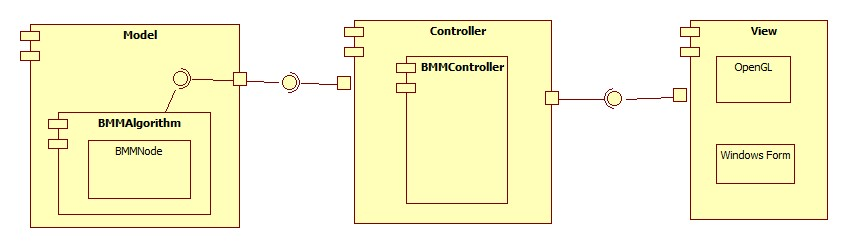
\includegraphics[width=\textwidth]{images/classes}
    \label{fig:classes}
    \caption[Component diagram of classes]{Component diagram of most important classes, forming the model-view-controller pattern.}
\end{figure}

\subsection{Model}

Model stores the data required for our algorithm, that is the input skeleton.
Model can be in six different states, five of which mirror the steps of base mesh algorithm.
The states are: skeleton editing, skeleton straightening, BNP generation, BNP refinement, BNP joining and final vertex placement.
To input a skeleton and display the corresponding generated base mesh only skeleton editing and final vertex placement would be adequate.
However the remaining states are useful for visualization of the algorithm.
The model is designed like a library, that means it is independent from view and controller and base mesh generation can be distributed as a library.

In skeleton editing state, the input skeleton is accessible for editing.
New nodes can be added to skeletal structure.
Existing nodes can be moved, their corresponding sphere can be specified, transformation matrices can be set and leaf nodes can be set to capsules or triangle fans.
Also cyclic edges between two nodes can be specified in this state.
Outside of this state user can not edit the input skeleton by any means.

After entering skeleton straightening state the preprocessing step skeleton straightening is executed and the resulting straightened skeleton is displayed.
User can inspect the effect that skeleton straightening has on the input skeleton.

Upon entering BNP generation state the corresponding algorithm stage is executed.
User can now see polyhedrons, corresponding to each branch node, generated by spherical Delaunnay triangulation.
User can inspect faces of generated polyhedrons and display their normals.

In BNP refinement state user can see refined and smoothed polyhedrons generated by our algorithm.
The refinement procedure can be changed, after which the algorithm will be recomputed and polyhedrons smoothed with different smoothing scheme will be shown to the user.

In BNP joining state the equally named step of our algorithm is executed.
User can see straight base mesh and display normals corresponding to its faces.
It is also possible to tessellate the straightened base mesh.
The tessellation factor is global and can be adjusted from GUI.
Since the last step of the algorithm was not yet executed, elliptical nodes would appear as spherical nodes.

After entering final vertex placement state, the last step of the algorithm is executed.
User can see the final output base mesh and adjust tessellation factor.
Elliptical node have their corresponding transformations applied.
After executing any step of the base mesh algorithm user can return to any previous state, which will re-execute the algorithm again.
Application work flow is depicted in Figure \ref{fig:states}.
Direct transitions between states represent steps of the base mesh algorithm.
Transitions through junction node represent the possibility to jump between any two states in the application.

\begin{figure}[h]
    \centering
    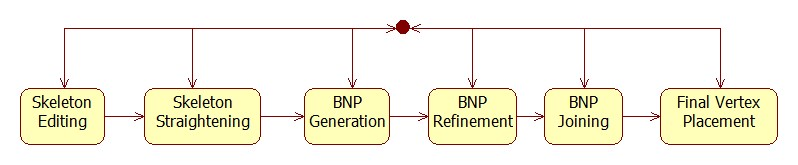
\includegraphics[width=\textwidth]{images/states}
    \label{fig:states}
    \caption[Model state diagram]{State diagram of model. Arrows between states show application work flow. Transition between any states is possible through the junction node.}
\end{figure}

\subsubsection{BMMNode}

BMMNode is main class of the model that holds the input skeleton.
It is represented as an oriented rooted graph.
The root of the graphs is stored in BMMAlgorithm class.
The steps of base mesh algorithm are implemented in BMMNode class as recursive functions.
The functions first process the root node and then continue, with its child nodes.
All necessary data for drawing, tessellation and subsequent algorithm steps are also accessed recursively from skeletons root. All important variables are stored directly in nodes: input skeleton node position, generated polyhedron, skinning weights and other attributes required for the execution of base mesh algorithm.

\subsubsection{BMMAlgorithm}

BMMAlgorithm class provides interface that hides the underlying oriented graph and implements states discussed previously.
All queries to BMMAlgorithm are forwarded to the root node, which recursively produces output, that BMMAlgorithm returns.
This way if we would later decide to change base mesh algorithm in any way basic functionality would still be accessible through BMMALgorithm.
Furthermore BMM algorithm computes certain pre and post processing that simplifies algorithms in BMMNode.
BMMAlgorithm implements the re-rooting algorithm, so we do not need to check for invalid parents in recursive functions.
The rooted oriented graph is stored twice in BMMAlgorithm.
One copy is used to execute the base mesh algorithm itself and the other copy is used to stores the input of the algorithm, so that it can be re-executed.

\subsection{View}

View consist of Windows form components and an OpenGL view.
Windows form components are managed by Visual Studio and we are synchronizing them with our controller.
Models state is displayed in a view with OpenGL 4.3 context.
Mouse interaction in OpenGL view is recorded by our GLInput class.

\subsubsection{OpenGL view}

OpenGL view periodically queries controller for changes in model.
If model changed its state, or input skeleton was modified OpenGL view reloads buffers with new data from the model.
Otherwise view displays previously stored data.
This reduces unnecessary commands to reload buffers with data that is already stored.
Buffers are filled with data and active OpenGL programs are selected depending on models state.

In skeleton input and skeleton straightening states, buffers are filled with lines connecting skeletal nodes and spheres corresponding to each node.
Elliptical nodes transformation matrices are also stored in buffers.
Two shader programs are used to render skeletal structures.
One is specifically designed for line drawing.
The other is designed for sphere drawing.
In order to reduce the amount of data required to be send to GPU during node rendering, only one model of an icosahedron is send to GPU.
This model is then tessellated and smoothed to resemble a sphere.
Corresponding model matrices are used to position the tessellated sphere at skeleton nodes position, with appropriate scale.

BNP generation and BNP refinement states also share the same shader programs.
Upon entering these states all polyhedrons are queried from the model.
The queried polyhedrons are converted from half edge representation to indexed face representation and stored in buffers on GPU.
The shader program, responsible for rendering of polyhedrons, features one-pass wire-frame rendering and uniform shading for each triangle.
This settings are useful for visualization of generated polyhedrons.

In the last two states BNP joining and final vertex placement, the generated base mesh is converted from half edge to indexed face.
Quadrilateral parts of the mesh are send as quadrilaterals to GPU for tessellation.
Shader program for base mesh rendering displays uniformly shaded faces and wire-frame.
The shader program is also capable of Linear Blend Skinning computations, that transform the input mesh.
Currently they are used only to revert transformations applied during skeleton straightening.

\subsubsection{GLInput}

When users clicks in OpenGL view the position in view and mouse button are registered.
Mouse position is then converted from 2D view coordinates to 3D camera coordinates.
A ray with origin at mouse 3D projection and direction from camera to mouse 3D projection is casted in the scene.
The process is shown in Figure \ref{fig:camera_selection}.
The mouse 2D location was mapped onto near plane and yellow ray was casted into the scene.
The first hit object is then selected.
Mouse actions are context dependant.

If the ray intersects a node the node is selected, its corresponding attributes are displayed in the inspector.
A selected node can be moved in the scene and this way its position attributes are updated.
With selected node user can create new nodes as child of selected node with middle click of the mouse.
Right clicking on a different node creates a cycle between selected and clicked node.
User can also rotated child nodes of a node.
In this mode left, right and middle clicks produce rotations around X, Y and Z axis respectively.

If after tracing the ray we do not encounter a node the resulting interaction is handled as rotations and translations of camera.
Camera is locked on a point and can be rotated around that point by right clicking in the scene.
A left click moves the point in a plane that is parallel to near plane of the camera.
Mouse wheel translates the camera along its view direction and therefore produces the effect of zooming in and out with the camera.

\begin{figure}[h]
    \centering
    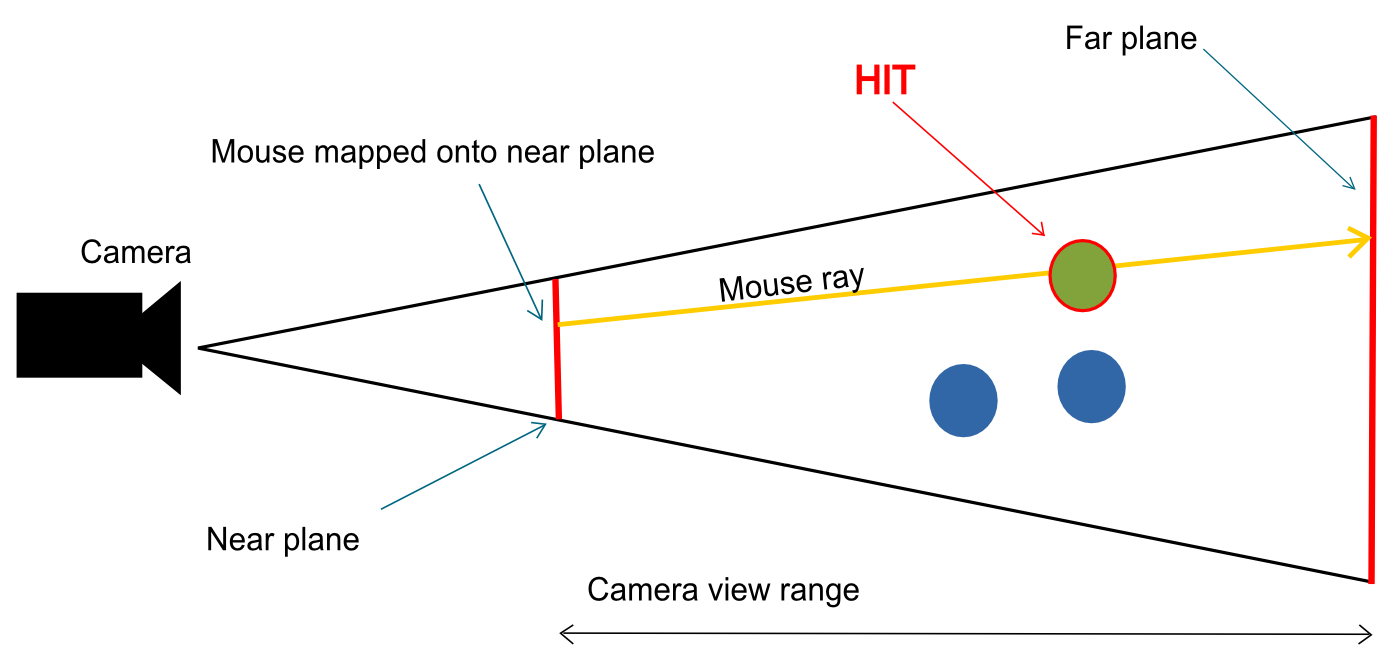
\includegraphics[width=\textwidth]{images/camera_selection}
    \label{fig:camera_selection}
    \caption[Camera selection]{Camera selection in 3D. Mouse 2D location is mapped onto near plane and a ray is casted through the scene. The first object hit by the ray is selected.}
\end{figure}

\subsection{Controller}

Controller is represneted by BMMController class.
BMMController connects model and view together by updating input forms with models data, providing OpenGL view with buffer data from the model and if new values are provided through input forms or mouse interaction, controller updates model accordingly.
Controller also handles file input and output.
When an input skeleton is loaded from a file, controller de-serializes objects saved in file and creates new BMMNode.
This new node is then set as the root for BMMAlgorithm.
BMMController is also capable of saving current skeleton into a file.
First controller queries BMMAlgorithm for skeletal representation through a provided interface.
Then controller serializes and stores the received skeletal structure.
Through a different interface, BMMController can query the generated base mesh, represented as Wavefront .obj and store it in a file.
Since controllers only interaction with model is providing input and output, it can be replaced at any time to accommodate for a different application.
For example in a library for base manifold mesh generation, where a one-shot algorithm would be desired, the controller would  send input skeleton to BMMAlgorithm.
Let BMMAlgorithm execute and return the generated base mesh either a Wavefron .obj suitable for storing or transferring to a different application, indexed face data structure suitable for rendering or in half edge data structure suitable for further mesh processing.

\section{GPU Shaders}

GPU shaders are used to program graphics hardware.
With shaders one can control the position of rendered vertices, lighting in scene and even compute certain calculation directly on GPU.
Since we are using OpenGL API to draw geometry, we are also using OpenGL Shading Language (GLSL) to program graphics hardware.
We are programming in GLSL version 430, which was released along with OpenGL 4.3.
We choose this version of GLSL because of two main reasons.
First, is that we wanted to use tessellation shaders that are available only in GLSL 400 and newer.
The second reason is that GLSL 430 offers various advantages to previous 4XX versions.
The main advantages comes from more extensive usage of layout qualifiers, which simplify application code.
New layout qualifiers allow us to bind texture units, shader uniforms and per-vertex attributes directly in shaders.
Application responsibility then becomes to send data to graphics card in appropriate order.
Shaders can be linked together to form a program that is responsible for drawing on GPU.
Each type of shader can be presented in a program only once.
GLSL version 430 features these types of shaders, listed in order of execution:
\begin{itemize}
	\itemsep-0.25em 
	\item \textbf{Vertex Shader} - must be implemented in every shader program. It purpus is to transform position of vertices sent to GPU.
	\item \textbf{Tessellation Control shader} - optional shader. Sets the level of tessellation that should be produced by hardware.
	\item \textbf{Tessellation Evaluation shader} - optional shader. Its main purpose is to adjust the position of vertices generated by tessellation.
	\item \textbf{Geometry shader} - optinal shader. Serves to generate new geometry directly on graphics hardware.
	\item \textbf{Fragment shader} - must be implemented in every shader program. Serves to defines the color of each fragment, from its material, lighting, etc.
\end{itemize}
We have implemented various specialized shaders.
In this section we will describe the most interesting and important of our implemented shaders.

\subsection{Skinning and Ellipsoid Nodes}

Linear Blend Skinning is a technique of animating characters.
As we described previously, we can compute final vertex placement as an animation, from straightened skeletons pose to input skeletons pose.
There are two attributes needed for Linear Blend Skinning: skinning matrices derived from rotation of bones around their degrees of freedom and per-vertex weights.
The weight resemble how much is a vertex influenced by each matrix.

For our case a vertex can not be influenced by more than two skinning matrices.
The first is rotation of a bone from bind pose (straightened skeleton) to reference pose (input skeleton).
The second matrix is matrix representing the rotation of the next bone from bind to reference pose.
This combination of matrices produces junctions that are not self collapsing.
Since we are using only two matrices per vertex, most of the matrices have assigned a weight of 0, so we can send as per-vertex data only weight for actually used matrices.
We are only sending weights for used matrices we also need to send index for each used matrix.
In practice GLSL reserves for each per-vertex attribute a space that can hold a vector of four components.
So we are sending four weights and four indices for each vertex, even though only two of them are used, this can potentially allows us to use mor complex skinning animations if we so desire.
Skinning matrices can be send to GPU in two ways.
The former is to send skinning matrices as uniforms, the latter is sending them in a texture.
Sending skinning matrices via textures is more general approach as a shader could be compiled just once and used for models with arbitrary number of bones.
However accessing uniforms in shaders is much faster that accessing textures and a shader needs to be compiled just once for each object.
Alternatively if we are sending matrices in shader uniforms we can reserve space needed for the object that requires most matrices and compile shaders only once.
For our implementation we only need do display one object, so we decided to send skinning matrices to GPU via shader uniforms, due to the efficiency of the method compared to textures.

We have implemented Linear Blend Skinning in vertex and tessellation evaluation shaders.
Vertex implementation resembles most a CPU implementation, as for the rest of the graphics pipeline vertex positions are equal.
We also implemented Linear Blend Skinning in tessellation evaluation shaders in order to compare visual results of skinning vertices after they have been tessellated.

\subsubsection{Vertex Shader Implementation}

The source code is shown in Listing \ref{lst:vert_skin}.
For each vertex we combine all matrices influencing said vertex into one.
We transform vertex and its normal with compound transformation matrix.
This way the vertex is transformed equivalently to a CPU implementation.
Since we also want to generate ellipsoid nodes, we send a transformation matrix for each node.
Because the number of nodes is the same as the number of skinning matrices, we can safely use an array of the same length for both skinning and transformation matrices.
Transformations are specific for each node, which means that transformation matrices do not need to be combined nor weighted.
To optimize the number of data send to GPU we store ids of skinning matrices in a specific order.
The first id is always the id of a transformation matrix that should be applied on currently precessed vertex.

\linespread{1.2}
\begin{lstlisting}[language=GLSL,caption={Linear Blend Skinning implemented in vertex shader},label={lst:vert_skin}]
/*                        Vertex Shader                      */ 
#version 430
//number of matrices filled in before compilation
#define SKINNING_MATRICES fill_in_skinnig_matrices_number
//input variables
layout (location = 0) in vec3 Position;
layout (location = 1) in vec3 Normal;
layout (location = 2) in ivec4 id;
layout (location = 3) in vec4 w;
//shader uniform variables
uniform mat4 MVPMatrix;
uniform mat4 SkinningMatrices[SKINNING_MATRICES];
uniform mat4 TransformMatrices[SKINNING_MATRICES];
//shader main function
void main(void) {
	vec4 pos = vec4(Position, 1.0);
	vec4 normal = vec4(Normal, 0.0);
	//skinning
	mat4 M = (w.x*SkinningMatrices[id.x]
		+ w.y*SkinningMatrices[id.y] 
		+ w.z*SkinningMatrices[id.z] 
		+ w.w*SkinningMatrices[id.w]);
	pos = M * pos;
	normal = M * normal;
	//ellipsoid transformations
	pos = TransformMatrices[id.x] * pos;
	normal = normalize(TransformMatrices[id.x] * normal);
	//output position
	gl_Position = MVPMatrix * pos;
}
\end{lstlisting} 
\linespread{1.5}

\subsubsection{Tessellation Evaluation Shader Implementation}

In tessellation evaluation shader new vertices and faces are generated.
For each tessellated patch we have access to the former vertices that existed before tessellation took place.
Each of this vertices has its corresponding matrices and weights assigned.
However the new vertices do not.
We used two approaches to propagate skinning information from original patch vertices to newly generated vertices.

According to patch vertex order shown in Figure \ref{fig:tess_patch}, we can apply skinning information corresponding to the second patch vertex to all newly generated vertices.
This way the new vertices would be oriented directly towards the last vertices of each patch.
Source code of this approach is shown in Listing \ref{lst:te_last_skin}.
Firs a matrix is determined depending on parameter $v$.
Vertices lying on patch borders have applied the same skinning transformations as patch vertices.
The new vertices do not use the second transformation matrix, because they are not directly joined to a different bone and do not need to be equally split between two bones.

\linespread{1.2}
\begin{lstlisting}[language=GLSL,caption={Linear Blend Skinning implemented in tessellation evaluation shader, using only skinning information from the first patch vertex.},label={lst:te_last_skin}]
vec3 skinningLastOnly(in vec4 pos, in float v, in ivec2 id0, in ivec2 id1, in vec2 w0, in vec2 w1, in mat4 SkinningMatrices[SKINNING_MATRICES]) {
	mat4 M;
	if (floatEqual(v, 0)) {
		//vertices from patch begining
		M = (w0.x*SkinningMatrices[id0.x] +
			 w0.y*SkinningMatrices[id0.y]);
	} else if (floatEqual(v, 1)) {
		//vertices from patch end
		M = (w1.x*SkinningMatrices[id1.x] +
			 w1.y*SkinningMatrices[id1.y]);
	} else {
		M = SkinningMatrices[ids1.x];
	}
	return M * pos;
}
\end{lstlisting} 
\linespread{1.5}

Second approach is averaging of all skinning data corresponding to patch vertices.
This effect produces smoother transitions between bones.
However smoother transitions limit the curvature of each bone, so they can deviate from the input skeleton, when compared to previously described skinning methods.
The source code is shown in Listing \ref{lst:te_avg_skin}.
The input vertex is transformed by each matrix and the combined to one vertex using skinning weights and its $v$ coordinate.

\linespread{1.2}
\begin{lstlisting}[language=GLSL,caption={Linear Blend Skinning implemented in tessellation evaluation shader, with avaraging of skinning information from all patch vertices.},label={lst:te_avg_skin}]
vec3 skinningAvarage(in vec4 pos, in float v, in ivec2 id0, in ivec2 id1, in vec2 w0, in vec2 w1, in mat4 SkinningMatrices[SKINNING_MATRICES]) {
	vec4 pos0, pos1;
	//lower patch skinning matrices
	pos0 = SkinningMatrices[id0.x] * pos;
	pos1 = SkinningMatrices[id0.y] * pos;
	vec4 t1 = w0.x*pos0 + w0.y*pos1;
	//upper patch skinning matrices
	pos0 = SkinningMatrices[id1.x] * pos;
	pos1 = SkinningMatrices[id1.y] * pos;
	vec4 t2 = w1.x*pos0 + w1.y*pos1;

	return (1-v)*t1 + v*t2;
}
\end{lstlisting} 
\linespread{1.5}

The resulting tessellated meshes are shown in Figure \ref{fig:tess_skin_comp}.
Mesh skinned in vertex shader Figure \ref{fig:tess_skin_comp} (a) produces visual artifacts at each node of the skeleton.
Last only tessellation evaluation skinning Figure \ref{fig:tess_skin_comp} (b) reduces visual artifacts and keeps the volume of the input.
Avarage tessellation evaluation shader skinning Figure \ref{fig:tess_skin_comp} (c) produces the smallest number of visual artifacts.

\begin{figure}[h]
    \centering
    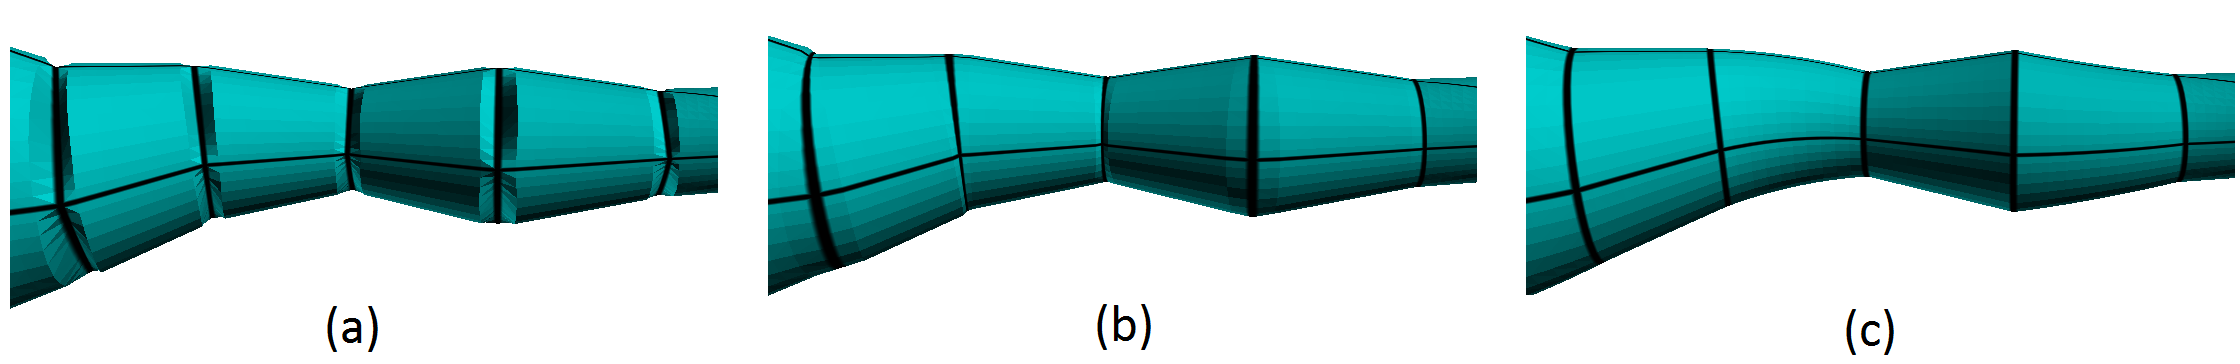
\includegraphics[width=\textwidth]{images/tess_comp}
    \label{fig:tess_skin_comp}
    \caption[Skinning and Tessellation]{Effects of selected skinning method on tessellation results. (a) vertex shader skinning; (b) last only tessellation evaluation shader skinning; (c) all average tessellation evaluation shader;}
\end{figure}

\subsection{Tessellation and Smoothing}

If tessellation is enabled OpenGL is rendering patches instead of triangles.
A patch can be composed of arbitrary number of vertices, however the number must be constant among all rendered patches.
Since we are tessellating quads our patch is composed from four vertices.
Our patch is depicted in Figure \ref{fig:tess_patch}.
Vertices forming the patch are in counter-clockwise order starting with v0.
Uv coordinates are displayed with blue and red respectively.
These coordinates are used to determine the position of new vertices generated during tessellation.

\begin{figure}[h]
    \centering
    \includegraphics[height=15em]{images/tess_patch}
    \label{fig:tess_patch}
    \caption[Tessellation patch]{A patch used to draw during tessellation. Patch vertices are marked with black, uv coordinates on patch are shown in blue and red respectively.}
\end{figure}

The new vertices lie on the same plane as the original quadrilateral.
Because of that in order to have any meaningful results, we also need to process the generated vertices.
We could use an already existing GPU subdivision algorithm for example subdivision approximation with Gregory patches \cite{gregory_patch}, or adaptive tessellation of subdivision surfaces presented in \cite{gpu_gems_2}.
However both of these algorithms are fairly complex, so we decided to use a simpler approach.

Each node has a defined sphere, so that between each pair of nodes lies a truncated cone.
We can sample the radius of truncated cone along its height, which corresponds to v coordinate and simply project each new vertex onto the truncated cone.
This way newly inserted vertices would have corresponding radius according to the input skeleton.
An example of such a shader is shown in Listing \ref{lst:tess_proj}.
However with this procedure the tessellated mesh gains volume, which could lead into self intersection.
In order to avoid this self intersection we are smoothing patches whose vertices have too sharp angles and therefore could potentially intersect with another patch.
We are using ease-in, ease-out and ease-in-out, depending on if the bottom patch vertices (v0, v3), upper patch vertices (v1, v2) or both have sharp angles with their neighbours respectively.
The sharpness of angles is computed by thresh holding the angle between normal of each vertex and v direction of current patch.
Another disadvantage of this approach are visual artifacts, that are produced when we are applying Linear Blend Skinning and were discussed previously.

\linespread{1.2}
\begin{lstlisting}[language=GLSL,caption={Tessellation evaluation shader projecting tessellated vertices onto truncated cone.},label={lst:tess_proj}]
/*               Tessellation Evaluation Shader              */ 
#version 430
//patch layout
layout(quads) in;
//per vertex attributes
in vec3 NodePosition[];
flat in int NodeID[];
//shader uniforms
uniform mat4 MVPMatrix;
layout(binding=0) uniform sampler2D Radiuses;
uniform int MaxID;

void main() {
    float u = gl_TessCoord.x, v = gl_TessCoord.y;
	//quads go in lower right -> upper right ->
	//upper left -> lower left
	vec3 a = mix(gl_in[0].gl_Position.xyz,
		     gl_in[3].gl_Position.xyz, u);
	vec3 b = mix(gl_in[1].gl_Position.xyz,
		     gl_in[2].gl_Position.xyz, u);
	vec3 position = mix(a, b, v);
	//get radiuses from texture
	float id0 = float(NodeID[0]) / float(MaxID);
	float id1 = float(NodeID[1]) / float(MaxID);
	float radius1 = texture(Radiuses, vec2(id0, id1)).r;
	float radius2 = texture(Radiuses, vec2(id1, id0)).r;
	float radius = mix(radius2, radius1, v);
	//project vertex onto cone
	vec3 dir = normalize(NodePosition[1]-NodePosition[0]);
	float projLength = dot(dir, position-NodePosition[0]);
	vec3 projection = NodePosition[0] + (dir * projLength);
	vec3 normal = normalize(position - projection);
	position = projection + (normal * radius);

	gl_Position = MVPMatrix * vec4(position, 1);
}
\end{lstlisting} 
\linespread{1.5}

\subsection{One-pass Wire-frame}

We have implemented one-pass wire frame rendering method as described in Single-pass Wireframe Rendering \cite{wireframe}.
This technique serves for many visualization purposes.
We can see triangles and quadrilaterals generated by our base mesh algorithm.
We can also display wireframe for new triangles generated during tessellation.
We have expanded upon the original idea and we are able to display differently colored wireframe for patches and tessellated triangles.

\section{Base Manifold Mesh Library}

Thanks to our interface based implementation of model, we are able to extract it from our application and build a stand alone library for base mesh generation.
Since input is handled by controller in our implementation a new controller had to be designed.
The new controller allows user to input his skeleton either as an object or via a file stored on his hard drive.
The loaded skeletal structure is then passed to BMMAlgorithm.
The base mesh generating algorithm is executed and output is provided to the user.
Depending on the selected output option either a Wevefron .obj file ready for storing on hard drive is provided to the user.
Alternatively a user can receive arrays containing positions of vertices, normals and other per-vertex attributes, along with a list of faces indexing into array of vertices.
This structures are OpenGL ready and can be directly loaded into a vertex array object and rendered.